\chapter{\label{lesson12}Движение по дуге}
{\bfseries Анонс:}\\\\
Алгоритм движение по дуге заданного радиуса. Алгоритм движения по дуге заданного радиуса и градусной меры.\\\\
{\bfseries Цели:}
\begin{itemize}
	\item{}{\bfseries Обучающие:} Добиться понимания и воспроизведения основных алгоритмов движения по дугам с заданными параметрами.
	\item{}{\bfseries Воспитательная:} Содействовать развитию аккуратности, терпения и настойчивости.\\
\end{itemize}	
{\bfseries Ход занятия:}\\\\
\begin{tabular}{lll}
	\hyperlink{lesson12x1}{1. Организационный момент} & Презентация & (15 мин)\\
	\hyperlink{lesson12x2}{2. Дуга заданного радиуса} & Практикум & (50 мин) \\
	\hyperlink{lesson12x3}{3. Дуга заданного радиуса и градусной меры} & Практикум & (50 мин) \\
\end{tabular}\\\\

{\hypertarget{lesson12x1}{\blackBlueText{I. Организационный момент}}}\\\\ 

В ходе этого занятия учащимся предстоит выполнить два больших самостоятельных практикума. Задания лучше выполнять в парах, на каждую пару полагается один набор конструктора и компьютер с RobotC.

Ввиду трудности поставленных задач, в ходе работы преподавателю необходимо непрерывно контролировать процесс, подсказывать и помогать каждой паре. По возможности следует содействовать обмену информацией  между учениками, подчеркнуть случаи взаимопомощи, однако все же не превращать занятие в коллективное творчество.

В начале занятия все команды собирают стандартную трехколесную тележку.\\\\

{\hypertarget{lesson12x2}{\blackBlueText{II.  Дуга заданного радиуса}}}\\\\ 

Наш робот умеет поворачивать на месте и ездить прямо. Теперь нужно научить его ездить по кривым. Самой простой кривой является дуга окружности, более того, любую более сложную гладкую кривую можно представить в виде комбинации дуг окружности разного диаметра. Поэтому наш следующий практикум посвящен движению по дуге окружности заданного радиуса.\\\\
Задача: Робот должен бесконечно ездить по окружности радиусом 1 метр.

{\slshape Стоит сначала дать детям возможность попробовать решить задачу самим, затем вывести всем вместе нижеследующие формулы и дать еще времени на самостоятельное дописывание и тест программы.}

Если оба колеса робота вращаются с одинаковой скоростью – робот едет по прямой. Пусть теперь скорости вращения колес различны и постоянны (\(V_{\mbox{\slshape внеш}}\) и \(V_{\mbox{\slshape внутр}}\)). Они относятся как  мощности подаваемые на моторы \(n_{\mbox{\slshape внеш}}\) и \(n_{\mbox{\slshape внутр}}\) . С другой стороны, поворачиваясь на угол \(\varphi\) колеса проходят пути \(\varphi R_{\mbox{\slshape внеш}}\) и \(\varphi R_{\mbox{\slshape внутр}}\) за одно и то же время.\\\\

\greenText{Схема движения тележки вид сверху с подписанными углами и расст}\\\\

Получается, что

\begin{equation}
\frac{n_{\mbox{\slshape внеш}}}{n_{\mbox{\slshape внутр}}}=\frac{V_{\mbox{\slshape внеш}}}{V_{\mbox{\slshape внутр}}}=\frac{\varphi R_{\mbox{\slshape внеш}}}{\varphi R_{\mbox{\slshape внутр}}}=\frac{R_{\mbox{\slshape внеш}}}{R_{\mbox{\slshape внутр}}}=\frac{R_{\mbox{\slshape внутр}}+l}{R_{\mbox{\slshape внутр}}}
\label{formulCirclesRadius}
\end{equation}  
где \(l\)~--- это расстояние между внешним и внутренним колесом тележки.

Важно отметить, что радиус окружности по которой будет двигаться тележка зависит лишь от отношения мощностей, а не от их абсолютных значений. Так, подача на моторы напряжений 100 и 50 приведет к такому же движению, что и подача напряжений 50 и 25. Различаться будут лишь скорости движения тележки, а не траектории.
При написании программы обычно задается мощность, подаваемая на одно из колес, а вторая вычисляется по формуле \ref{formulCirclesRadius}.
\clearpage
\begin{figure}[h!]
	\begin{center}
		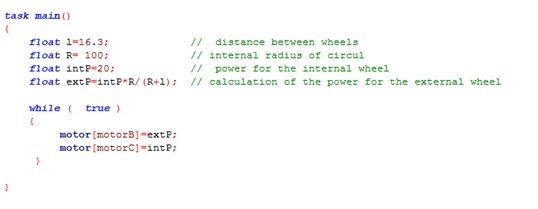
\includegraphics[width=0.98\linewidth]{chapters/chapter12/images/1}
		\caption{}
		\label{ris:image12x1}
	\end{center}
\end{figure}

{\hypertarget{lesson1232}{\blackBlueText{III. Дуга заданного радиуса и градусной меры}}}\\\\	
Задача: Робот должен проехать четверть окружности радиуса 1 метр.\\
Возможное решение:

\begin{figure}[h!]
	\begin{center}
		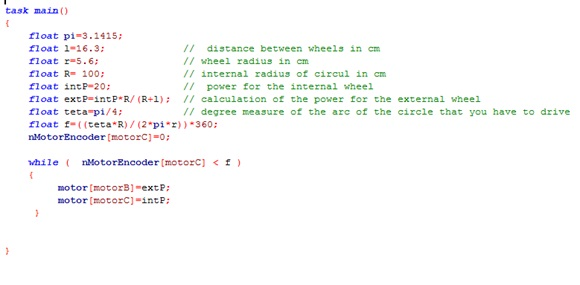
\includegraphics[width=0.98\linewidth]{chapters/chapter12/images/2}
		\caption{}
		\label{ris:image12x2}
	\end{center}
\end{figure}	

{\slshape По сути своей задача представляет собой комбинацию двух, уже известных: проехать известное расстояние и ехать по дуге известного радиуса. Поэтому здесь лучше больше внимания уделить самостоятельной работе детей, подсказывая и направляя каждого в отдельности. Использование переменных и формул расчета обязательно.
	
Задача так же является отличным маркером усвоения материала последних занятий. Если большинство учащихся даже с подсказками не смогли справиться с задачей, значит необходимо еще раз подробнее разобрать вопросы движения по окружности.}